\section{Tecnologie}\label{chap:Tecnologie}
\subsection{Elenco delle tecnologie utilizzate}
L'azienda utilizza diversi strumenti sia per lo sviluppo, che per lo svolgimento dei normali processi aziendali.
\begin{itemize}
    \item \textbf{Portatili}: ad ogni impiegato viene messo a disposizione un portatile con Windows 10 o 11, il sistema 
          operativo di Microsoft o all'occorrenza un Mac con macOS, il portatile sviluppato da Apple con il suo sistema operativo proprietario;
    \item \textbf{Dispositivi \textit{mobile}}: all'interno dell'azienda troviamo molti dispositivi \textit{mobile} con diversi sistemi operativi e dimensioni 
          dello schermo, usati per il \textit{testing} delle applicazioni Android e iOS;
    \item \textbf{Microsoft Office 365}: servizio in abbonamento di Microsoft che include diversi software come Word e PowerPoint;
    \item \textbf{Zimbra}: sistema di posta elettronica utilizzato dall'azienda, durante il mio stage è stato cambiato in favore di un'integrazione di Zimbra 
          con Outlook;
    \item \textbf{Bitbucket}: strumento per la gestione della versione Git basato sul \textit{web}, che consente di creare 
          \textit{repository} pubbliche o private per caricare il proprio codice e gestirlo in modo collaborativo con il proprio 
          \textit{team};
    \item \textbf{Jira}: \textit{suite} di \textit{software} proprietari per il tracciamento delle segnalazioni sviluppato
           da Atlassian, che consente il \textit{bug tracking} e la gestione dei progetti;
    \item \textbf{Confluence}: strumento che permette ai \textit{team} di condividere e organizzare documenti e contenuti 
          in un ambiente centralizzato e strutturato;
    \item \textbf{3CX}: centralino telefonico PBX (\textit{Private Branch Exchange}), ovvero una rete telefonica privata utilizzata all'interno di un'azienda 
          o organizzazione. Gli utenti del sistema telefonico PBX possono comunicare internamente ed esternamente, tramite il classico telefono fisso o 
          chat da \textit{smartphone}. Questo sistema permette anche di effettuare video chiamate e di scambiarsi messaggi all'interno di \textit{chat};
    \item \textbf{Visual Studio}: Si tratta di un ambiente di sviluppo integrato completo (\gls{ide}) che è possibile usare per scrivere, modificare, 
          eseguire il \textit{debug} e compilare codice. Visual Studio include \textbf{compilatori, strumenti di completamento del codice, 
          controllo del codice sorgente, estensioni} e molte altre funzionalità per migliorare ogni fase del processo di sviluppo \textit{software};
    \item \textbf{Visual Studio Code}: \textit{editor} di codice sorgente particolarmente leggero ed estensibile grazie ad una gamma di estensioni 
          che è possibile integrargli. È inoltre \textit{open source} e compatibile con una vasta gamma di sistemi operativi;
    \item \textbf{SQL Server Management Studio (SSMS)}: è un ambiente integrato per la configurazione, la gestione e l'amministrazione di tutti i componenti, 
          le istanze e i database all'interno di Microsoft SQL Server. SSMS include sia \textit{editor} di \textit{script} che strumenti grafici che lavorano con 
          oggetti e funzionalità del \textit{server}.
\end{itemize}
L'azienda utilizza una vasta gamma di linguaggi di programmazione, \textit{framework} e librerie per diversi motivi. Alcuni di questi includono l'acquisizione 
e l'adattamento di codice sorgente da altre aziende, il fatto che il codice sia stato scritto molti anni fa con tecnologie ormai obsolete, e la necessità di utilizzare 
linguaggi specifici per soddisfare esigenze particolari. Tuttavia, l'azienda si impegna a uniformare quanto più possibile i linguaggi e a ridurre il numero di tecnologie in 
uso, al fine di semplificare e rendere più efficiente la gestione delle risorse tecnologiche. Oltre a quelle che ho usato per il mio progetto (che verranno discusse 
più approfonditamente nel capitolo TODO 2.4.1) queste sono alcune delle tecnologie che l'azienda usa per lo sviluppo dei suoi prodotti.
\begin{itemize}
    \item \textbf{Angular}: \textit{framework} per lo sviluppo di \gls{webapp} basato su TypeScript, sviluppato e mantenuto da Google;
    \item \textbf{Librerie Dev Express}: Dev Express è un'azienda incentrata sulla creazione di librerie di componenti grafici di cui le più famose sono 
          Blazor e MAUI. Queste librerie sono supportate per lo sviluppo in React, Angular e Vue;
    \item \textbf{FoxPro}: un sistema di gestione di \textit{database} e un linguaggio di programmazione procedurale orientato agli oggetti. Originariamente sviluppato 
          da Fox Software e successivamente acquisito da Microsoft. 
\end{itemize}
\subsection{Integrazione delle tecnologie con i processi aziendali}
\begin{figure}[H]
      \centering
      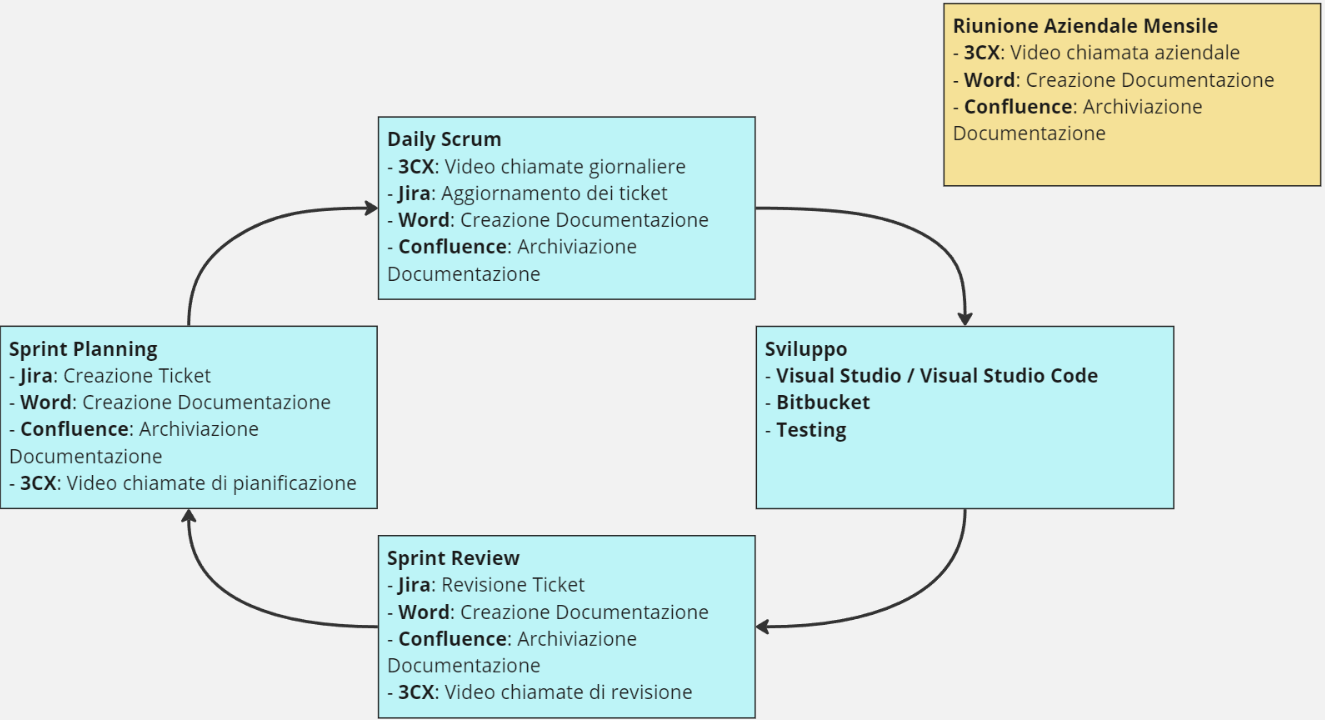
\includegraphics[alt={metodologie e tecnologie}, width=\textwidth]{img/integrazione metodologie strumenti.png}
      \caption[Integrazione metodologie e tecnologie]
              {Integrazione metodologie e tecnologie.}
      \label{fig:integrazione tecnologie e metodologie}
  \end{figure}
Come mostrato in figura \ref{fig:integrazione tecnologie e metodologie} l'applicazione del \textit{framework} Scrum richiede 
l'impiego di diverse tecnologie:
\begin{itemize}
      \item \textbf{Documentazione}: a seguito dei \textit{meeting} aziendali viene prodotto un documento che può 
            avere diverse finalità: trascrivere gli \textbf{argomenti dell'incontro}, le \textbf{difficoltà incontrate e le soluzioni da 
            applicare per correggerle} o \textbf{semplici appunti}. Gli sviluppatori usano quindi Word per redarre la documentazione 
            data la sua estrema semplicità e la velocità con la quale si possono produrre tali documenti;
      \item \textbf{Archiviazione di documenti}: eccezion fatta per gli appunti personali, la documentazione richiede di 
            essere condivisa e organizzata. Nonostante in {\company} esista una serie di cartelle di rete accedibili tramite 
            il \textit{file manager} di Windows, questa soluzione risulta inadeguata allo scopo in quanto povera di funzionalità 
            e personalizzazioni. Confluence permette non solo di organizzare la documentazione in una serie di \textit{directory 
            online} in modo da rendere i documenti sempre consultabili, ma permette anche di definire una serie di privilegi per 
            consentire o meno l'accesso alla documentazione.
      \item \textbf{Comunicazione}: 3CX agisce come canale di comunicazione per la maggior parte delle comunicazioni interne. 
            È il luogo dove si svolgono i \textit{meeting}, fondamentali per mantenere il \textit{team} coordinato, ma permette 
            anche di effettuare chiamate e scrivere in \textit{chat} confinando la maggior parte delle comunicazioni in un unico 
            luogo. Ovviamente anche le \textit{mail} sono un valido strumento di comunicazione, ed infatti viene usato Zimbra 
            per comunicare con persone esterne all'azienda o per alcune mail interne (\textbf{comunicazioni di servizio, 
            \textit{reminder}}, ecc.). Quindi 3CX viene usato maggiormente per i \textit{meeting} o per un tipo di 
            comunicazione veloce ed informale, mentre il servizio di posta elettronica viene usato principalmente 
            per comunicazione con persone esterne all'azienda. Ovviamente i clienti che hanno necessità di assistenza 
            possono chiamare l'assistenza tramite il numero di telefono che viene loro fornito per mettersi in contato con 
            uno dei tecnici del reparto assistenza;
      \item \textbf{Sviluppo}: Per quanto riguarda lo sviluppo gli strumenti utilizzati e le tecnologie impiegate variano 
            a seconda del progetto a cui lo sviluppatore sta lavorando o da preferenze personali (come nel caso del 
            sistema operativo utilizzato nel proprio \textit{computer}). Anche per quanto riguarda l'editor viene lasciata 
            libertà di scelta, personalmente per lo sviluppo di API in .NET (le tecnologie che ho impiegato per lo sviluppo del 
            progetto verranno discusse in un capitolo a parte TODO 3.1) ho preferito utilizzare Visual Studio perché offre 
            molti strumenti di supporto e \textit{debug} integrati. Per quanto riguarda lo sviluppo del \textit{frontend} ho 
            preferito utilizzare Visual Studio Code perché più leggero, personalizzabile.
      \item \textbf{Testing}: anche qui gli strumenti utilizzati dipendono dal progetto che si sta sviluppando. Nel mio 
            caso ho utilizzato uno \textit{smartphone e tablet} Android per testare l'applicazione nel suo insieme e la 
            piattaforma Swagger per testare manualmente le API (le tecnologie che ho impiegato per lo sviluppo del 
            progetto verranno discusse in un capitolo a parte TODO 3.1, mentre per la descrizione accurata di come ho 
            effettuato il testing del codice consultare il capitolo TODO 3.6). Riporto per completezza che per 
            quanto riguarda il \textit{testing} di applicazioni Android è possibile emulare un dispositivo con gli 
            strumenti offerti dallo strumento di sviluppo Android Studio e installare l'applicazione su questo \textit{device} 
            virtuale. Il problema di questo strumento è che richiede computer con prestazioni molto alte per funzionare 
            in maniera fluida altrimenti rischia di paralizzare l'elaboratore. Non sono sicuro che sia utilizzato dagli 
            sviluppatori di {\company} quindi ho evitato di includerlo nelle tecnologie utilizzate;
      \item \textbf{Collaborazione e gestione del codice}: Bitbucket viene utilizzato come piattaforma per depositare il codice 
            sorgente e gestire lo sviluppo collaborativo. Qui gli sviluppatori caricano il loro 
            codice suddiviso in \textit{repository} per ogni progetto. Ogni \textit{repository} vede diversi 
            \textit{branch} attivi: \textbf{\textit{main}} che contiene l'ultima versione rilasciata al pubblico del software, 
            \textbf{\textit{develop}} ovvero il \textit{branch} di lavoro dove nascono e confluiscono tutti i 
            \textit{feature branch} prima di effettuare il rilascio in \textit{main}, i \textbf{\textit{feature branch}} che 
            viene creato dal programmatore per sviluppare una specifica funzione del programma che sarà, una volta 
            terminata e testata, aggiunta in \textit{develop};
      \item \textbf{Gestione dei progetti}: Jira è una piattaforma particolarmente utile per pianificare i vari 
            compiti da svolgere nello \textit{sprint} e assegnarli ai vari componenti del \textit{team} di sviluppatori. 
            Questi compiti sono chiamati \textit{ticket} e possono essere di diverso tipo: \textbf{\textit{epic}} che rappresentano 
            grosse porzioni di lavoro e sono quindi usate come raccolte di \textit{ticket}, \textbf{\textit{task}} il singolo 
            compito che deve essere completato e \textbf{\textit{bug}} che rappresenta una problematica da risolvere.
            I \textbf{\textit{bug}} possono essere avere diverse origini: gli sviluppatori stessi nel caso in cui si accorgano 
            di un difetto di programmazione o da i clienti che telefonando all'assistenza riportano il problema, 
            quindi il tecnico riporterà la problematica al \textit{project manager} che creerà la \textit{task}. Jira offre inoltre 
            molti altri strumenti per la gestione di metodologie Agile come la possibilità di creare diagrammi di Gantt, che 
            permettono di avere una rappresentazione visiva delle attività programmate nel tempo, aiutando il \textit{team} 
            a comprendere meglio la sequenza delle attività, o la definizione di un \textit{backlog}, ovvero una lista con le task 
            rimaste incompiute durante gli \textit{sprint} precedenti;
\end{itemize}